\documentclass[11pt, a4paper, DIV=12]{scrartcl}

% useful packages 
\usepackage{mathtools}
\usepackage{physics}
\usepackage{graphicx}					  
\graphicspath{{figs/}}



\usepackage{amssymb}
\usepackage{amsmath}
\usepackage{hyperref}
\usepackage[separate-uncertainty=true]{siunitx}
\usepackage{xcolor}
\usepackage{braket} % easy braket notation
\usepackage{enumitem}
\usepackage{booktabs}
\usepackage{here}
\usepackage{cprotect}

\usepackage[backend=biber, sorting=none]{biblatex}
\bibliography{refs.bib}

% \numberwithin{equation}{section}

\title{Form factor of a two-boson bound state}
\date{\today}
\author{Harilal Bhattarai \& Marcel Schindler}
\begin{document}
	\maketitle
	
\section{Introduction}
The  bound state is a quantum state of a particle subject to a potential such that the particle has a tendency to remain localized in one or more regions of space. 

In this exercise, we would like to study the properties of bound states of two bosons. We assume that the bound state problem was solved for the OBE using several cutoffs. Thereby, the interactions have been tuned so that our two-boson system corresponds to the deuteron bound state in nuclear physics and reproduce the experimentally known binding energy of E = -2.225 MeV.

\section{Solution of questions}
\textbf{Question No 2}
\begin{equation}
F(\vec{q}^2)=\int d^3 q\prime ~\psi ^* (\vec{p}\prime) ~\psi(\vec{p}\prime - \frac{1}{2}\vec{q})
\label{Equ:QN1}
\end{equation}
To verify,
\begin{equation}
F(\vec{q}^2)= ~ 2\pi\int dp ~p\prime ^2 \int_{-1}^{1} dx ~ Y_{lm_{z}}(\hat{p}\prime) ~ Y_{lm_{z}}(\vec{p}\prime - \frac{1}{2}\vec{q})  ~\psi^{*}_{lm_{z}} (\vec{p}\prime) ~\psi_{lm_{z}}(\vec{p}\prime - \frac{1}{2}\vec{q})
\label{Equ:QN2}
\end{equation}
We have to use the momentum $ \vec{p}\prime = (\vec{p}\sqrt{1-x^2}, 0, p\prime x)$, $ \vec{q}=q \hat{e}_{z}$ and the solid angle integration can be simplified to the integration over $ x= \cos(\theta) $. Also, we have

\begin{equation}
	\psi(\vec{p})= \sum_{l, m} \psi_{l}(|p|) ~ Y_{lm}(\hat{p})
\end{equation}
Since the angular momentum is consvered all other sum parts expect for given $l$ and $m_z$ vanishes. Also notice that we have no $\phi$ dependance, so we can integrate easily over $\phi$:
i.e.
\begin{align}
F(\vec{q}^2)=& \int d^{3}\vec{p}\prime~\psi^{*}_{lm_{z}} (|p\prime|) ~ Y_{lm_{z}}(\hat{p}\prime) ~\psi_{lm_{z}}(|\vec{p}\prime - \frac{1}{2}\vec{q}|) Y_{lm_{z}}(|\vec{p}\prime - \frac{1}{2}\vec{q}|)\\
=& \int_{0}^{\infty} d\vec{p} ~ p^{2}\prime ~ \int_{0}^{2 \pi} d\phi ~ \int_{0}^{\pi} d\theta \sin\theta ~\psi^{*}_{lm_{z}} (|p\prime|) ~ Y_{lm_{z}}(\hat{p}\prime) ~\psi_{lm_{z}}(|\vec{p}\prime - \frac{1}{2}\vec{q}|) Y_{lm_{z}}(|\vec{p}\prime - \frac{1}{2}\vec{q}|)\\
=& 2\pi ~\int_{0}^{\infty} dp\prime ~ p^{2}\prime ~\int_{-1}^{1}d x~\psi^{*}_{lm_{z}} (|p\prime|) ~ Y_{lm_{z}}(\hat{p}\prime) ~\psi_{lm_{z}}(|\vec{p}\prime - \frac{1}{2}\vec{q}|) Y_{lm_{z}}(|\vec{p}\prime - \frac{1}{2}\vec{q}|)
\end{align}

\textbf{Question No 4}\\
To check the numerical of our result, accuracy We have used the wave function for $\lambda=1200 $  MeV and selected momentum transfers $ |q| $ in the range up to $ 10 ~ fm^{-1} $. Especially with
respect to the number of grid points used for angular integration we got the plot as in figure \ref{fig:1}.
\begin{figure}[H]
	\centering
	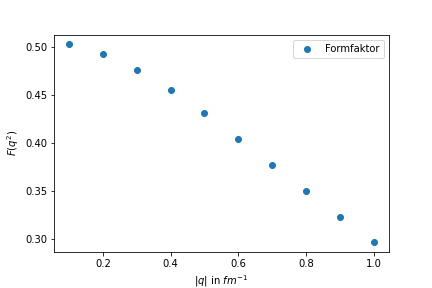
\includegraphics[width=0.6\linewidth]{problem4.png}
	\caption{ The distribution of form factor.}
	\label{fig:1}
\end{figure}
We can see that this plot is not quite correct because for $q=0$ the form factor should be 1. We also vary the grid points such that the change in value is only at the third significant position.\\
\textbf{Question No 4}\\
In the follwoing we plottet the form factor for different cutoffs $\Lambda$. Which you can see in \ref{fig:2}.
\begin{figure}[H]
	\centering
	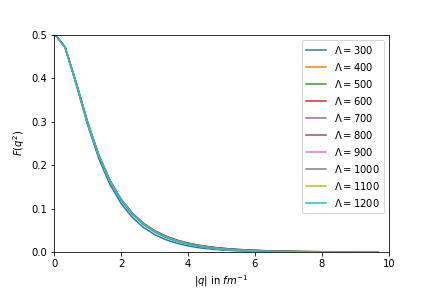
\includegraphics[width=0.49\linewidth]{problem6.png}
	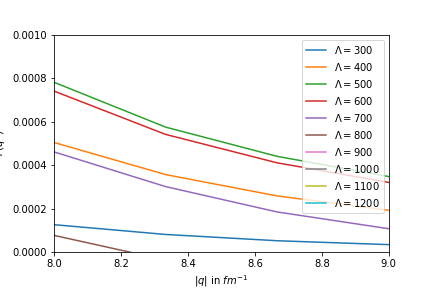
\includegraphics[width=0.49\linewidth]{problem6_2.png}
	\caption{Form factors for different cutoffs}
	\label{fig:2}
\end{figure}
We can see some differences but they are quite low and random. So we cannot really say one is bad or good. This of course can be explain by the fact that sth is still wrong in the calculation of the form factor.\\
\begin{thebibliography}{12}
\bibitem{exercise-sheet} 
Thomas Luu, Andreas Nogga, Marcus Petschlies and  Andreas Wirzba, Exercise-sheet, 2020. 
\end{thebibliography}	
\end{document}